\documentclass[
    margin=1in,
    innermargin=-4.5in,
]{tikzposter}

% Choose size here
\geometry{paperwidth=23.4in,paperheight=33.11in} % A1 portrait full-content layout
% \geometry{paperwidth=33.11in,paperheight=23.4in} % A1 landscape
% \geometry{paperwidth=33.11in,paperheight=46.81in} % A0 portrait

\usepackage[utf8]{inputenc}
\usepackage[T1]{fontenc}
\usepackage{csquotes}
\usepackage{amsmath} 
\usepackage{amsfonts}
\usepackage{amsthm}
\usepackage{amssymb}
\usepackage{mathrsfs}
\usepackage{graphicx}
\usepackage[export]{adjustbox}
\usepackage{tcolorbox}
\usepackage[font=scriptsize,labelfont=bf]{caption}
\usepackage{enumitem}
\usepackage{booktabs}
\usepackage{multirow}
\usepackage{array}
\usepackage{bm}
\usepackage{bbm}
\usepackage{tikz}
\usetikzlibrary{arrows.meta, positioning, shapes.geometric}
\usepackage[backend=biber,style=numeric]{biblatex}
\usepackage{glasgow-poster-theme}

\makeatletter
% Full-content layout: A1 portrait with conservative safe margins.
\setlength{\TP@visibletextwidth}{21.6in}
\setlength{\TP@visibletextheight}{31.6in}
\makeatother

\addbibresource{refs.bib}

% Set theme parameters
\tikzposterlatexaffectionproofoff
\usetheme{UniGlasgowTheme}
\usecolorstyle{UniGlasgowStyle}

% Light blue academic palette:
% reduce the visual weight of the original dark title bars while preserving hierarchy.
% Reference-style palette: slim navy bars with clean white content areas.
\colorlet{blocktitlebgcolor}{blue!55!black}
\colorlet{blocktitlefgcolor}{white}
\colorlet{blockbodybgcolor}{white}
\colorlet{blockbodyfgcolor}{black}
\colorlet{innerblocktitlebgcolor}{blue!55!black}
\colorlet{innerblocktitlefgcolor}{white}
\colorlet{innerblockbodybgcolor}{blue!5}
\colorlet{innerblockbodyfgcolor}{black}

% Reference-style slim full-width section bars.
\defineblockstyle{LightSlimTitleBar}{
    titlewidthscale=1,
    bodywidthscale=1,
    titlecenter,
    titleoffsetx=0pt,
    titleoffsety=0pt,
    bodyoffsetx=0pt,
    bodyoffsety=5.0mm,
    bodyverticalshift=5.0mm,
    roundedcorners=2,
    linewidth=0.4pt,
    titleinnersep=3.0mm, % keep a slim title bar while preserving vertical text clearance
    bodyinnersep=3.0mm
}{
    \draw[
        fill=blockbodybgcolor,
        draw=none
    ] (blockbody.south west) rectangle (blockbody.north east);
    % Draw the title bar last so the body area cannot cover the lower edge of the title text.
    \draw[
        fill=blocktitlebgcolor,
        draw=blue!55!black,
        line width=\blocklinewidth,
        rounded corners=\blockroundedcorners
    ] (blocktitle.south west) rectangle (blocktitle.north east);
}
\useblockstyle{LightSlimTitleBar}

% Use a Times New Roman-like font family for a formal academic style.
% Compile with pdfLaTeX. If you use XeLaTeX and have Times New Roman installed,
% you may replace these two lines with fontspec settings.
\usepackage{newtxtext}
\usepackage{newtxmath}
\renewcommand{\vec}[1]{\bm{#1}}
\newcommand{\Tr}{\text{Tr}}
\newcommand{\sectionbar}[1]{\normalsize\bfseries\raisebox{-0.08ex}{\strut #1}}
\setlist[itemize]{leftmargin=1.0em,itemsep=0.05em,topsep=0.08em,parsep=0pt,partopsep=0pt}

% ---------------------------------------------------------------------
% Poster information
% ---------------------------------------------------------------------
\title{\parbox{0.94\linewidth}{\centering
{\Large\bfseries\mbox{An Automatic Four-Part Harmony Grading System}}\\[0.12em]
{\normalsize\bfseries Integrating Deep Learning-Based Optical Music Recognition and Rule-Based Analysis}
}}

\author{\parbox{0.92\linewidth}{\centering
    {\normalsize MA, SIAO-SHIH}\\[0.10em]
    {\small Advisor: Ming-Hsueh Lin}
}}

\institute{\parbox{0.92\linewidth}{\centering
    {\small Arete Honors Program}\\[0.05em]
    {\small National Yang Ming Chiao Tung University}
}}

\makeatletter
\renewcommand\TP@maketitle{%
    \centering
    \begin{minipage}{0.96\linewidth}
        \centering
        {\color{titlefgcolor}\@title\par}
        \vspace{0.12em}
        {\color{titlefgcolor}\@author\par}
        \vspace{0.04em}
        {\color{titlefgcolor}\@institute\par}
    \end{minipage}
    \par\vspace{0.00cm}
}
\makeatother

% ---------------------------------------------------------------------
% Helper styles
% ---------------------------------------------------------------------
\newcommand{\compactblock}[2]{%
    \par\vspace{0.36cm}%
    \noindent\tcbox[
        on line,
        colback=blue!20,% lighter background for less visual weight
        colframe=blue!50!black,
        boxrule=0.4pt,% subtle border
        arc=1.5pt,% smaller corner radius
        left=2.5mm,
        right=2.5mm,
        top=0.8mm,
        bottom=0.8mm
    ]{\color{blue!50!black}\small\bfseries #1}%
    \par\vspace{0.20cm}%
    #2%
    \par\vspace{0.24cm}%
}

\tikzset{
    pipelinebox/.style={
        rectangle,
        rounded corners=6pt,
        draw=blue!50!black,
        fill=blue!10, % slightly stronger than very light background
        thick,
        minimum height=1.15cm,
        text width=7.2cm, % narrower to avoid overflow
        align=center,
        font=\small\bfseries
    },
    methodbox/.style={
        rectangle,
        rounded corners=6pt,
        draw=blue!50!black,
        fill=blue!10,
        thick,
        minimum height=0.95cm,
        text width=2.25cm,
        align=center,
        font=\scriptsize\bfseries
    },
    layerlabel/.style={
        rectangle,
        rounded corners=4pt,
        draw=blue!50!black,
        fill=blue!20,
        text=blue!50!black,
        minimum height=0.72cm,
        text width=2.55cm,
        align=center,
        font=\scriptsize\bfseries
    },
    pipelinearrow/.style={
        -{Latex[length=5mm]},
        thick,
        draw=blue!50!black
    }
}

\begin{document}
\maketitle
\centering
\nocite{*} % Print all bibliography entries in refs.bib even if they are not cited inline.


\begin{columns}
% =====================================================================
% Left column: problem, method, model, rules
% =====================================================================
\column{0.49}

\block{{\sectionbar{Abstract \& Motivation}}}{
\scriptsize
Four-part harmony is a fundamental component of music theory education.
Students must simultaneously consider voice leading, chord spacing, doubling,
leading-tone resolution, cadence structure, and other harmonic constraints.
Traditional grading depends heavily on expert teachers and often requires
substantial time for manual correction.

\vspace{0.12cm}
Although Optical Music Recognition (OMR) systems can recognize music notation
from score images, most existing systems focus on symbol detection or score
transcription rather than harmony-specific analysis and explainable learning
feedback.

\vspace{0.10cm}
\begin{tcolorbox}[colback=blue!6,colframe=blue!45!black,title=Key Problem]
\scriptsize
How can a system convert a score image into localized and explainable
four-part harmony feedback for student learning?
\end{tcolorbox}
}

\block{{\sectionbar{Objectives \& Contributions}}}{
\scriptsize
This study aims to design an automatic four-part harmony grading system that
integrates deep learning-based Optical Music Recognition with rule-based
harmony analysis.

\vspace{0.10cm}
\begin{tabular}{p{0.48\linewidth}p{0.48\linewidth}}
\textbf{Objectives} & \textbf{Contributions} \\
\begin{itemize}
    \item Detect music notation symbols from score images using a YOLO-based OMR model.
    \item Convert detected symbols into structured four-part harmony snapshots.
    \item Analyze common harmony errors through a rule-based engine.
    \item Present localized errors with rule explanations and correction suggestions.
\end{itemize}
&
\begin{itemize}
    \item A system architecture connecting score recognition and harmony rule analysis.
    \item A structured representation for four-part harmony snapshots.
    \item A rule-based engine for representative voice-leading and chord-configuration errors.
    \item A web-based prototype demonstrating the grading workflow.
\end{itemize}
\end{tabular}
}

\block{{\sectionbar{System Design \& Pipeline}}}{
\footnotesize
\begin{center}
\begin{tikzpicture}[node distance=0.46cm and 0.28cm]
    \node[layerlabel] (inputlabel) {Input};
    \node[methodbox, right=0.55cm of inputlabel, text width=6.2cm] (input) {Score Image};

    \node[layerlabel, below=0.72cm of inputlabel] (omrlabel) {Deep Learning-\\Based OMR};
    \node[methodbox, right=0.55cm of omrlabel, text width=2.8cm] (prep) {Image\\Preprocessing};
    \node[methodbox, right=of prep, text width=2.8cm] (detect) {YOLO Symbol\\Detection};
    \node[methodbox, right=of detect, text width=2.8cm] (assembly) {Symbol-to-\\Voice Assembly};

    \node[layerlabel, below=0.72cm of omrlabel] (rulelabel) {Rule-Based\\Analysis};
    \node[methodbox, right=0.55cm of rulelabel, text width=2.8cm] (snapshot) {ChordSnapshot\\Representation};
    \node[methodbox, right=of snapshot, text width=2.8cm] (rules) {Harmony Rule\\Engine};
    \node[methodbox, right=of rules, text width=2.8cm] (feedback) {Localized\\Feedback};

    \draw[pipelinearrow] (input) -- (prep);
    \draw[pipelinearrow] (prep) -- (detect);
    \draw[pipelinearrow] (detect) -- (assembly);
    \draw[pipelinearrow] (assembly) -- (snapshot);
    \draw[pipelinearrow] (snapshot) -- (rules);
    \draw[pipelinearrow] (rules) -- (feedback);
\end{tikzpicture}
\scriptsize
\captionof{figure}{Overall workflow of the proposed four-part harmony grading system.}
\end{center}

\vspace{0.08cm}
The architecture separates visual recognition from musical reasoning, allowing
the OMR model and the harmony rule engine to be improved independently.
}

\block{{\sectionbar{Rule-Based Harmony Analysis}}}{
\scriptsize
The rule engine receives a sequence of chord snapshots. Each snapshot contains
the pitch, measure, beat, and voice assignment of Soprano, Alto, Tenor, and
Bass parts.

\vspace{0.03cm}
\begin{center}
\tiny
\begin{tabular}{>{\bfseries}p{0.7cm}p{3.5cm}p{8.4cm}}
\toprule
ID & Rule Type & Description \\
\midrule
M1 & Melodic leap constraints & Detects excessive leaps, sevenths, and augmented or diminished melodic intervals. \\
V1 & Voice crossing and overlap & Checks whether adjacent voices cross or overlap between consecutive chords. \\
P1 & Parallel fifths and octaves & Detects parallel perfect fifths and octaves between any pair of voices. \\
P2 & Hidden fifths and octaves & Checks direct motion into perfect intervals, especially between outer voices. \\
D1 & Triad doubling and omission & Verifies root, third, fifth, and leading-tone treatment in triads. \\
L1 & Leading-tone resolution & Checks whether leading tones resolve properly to the tonic. \\
\bottomrule
\end{tabular}
\captionof{table}{Representative harmony rules implemented in the rule engine.}
\end{center}

\vspace{0.02cm}
Each detected issue is mapped to a rule identifier, severity level, involved
voices, score location, explanation, and correction suggestion.
}

% =====================================================================
% Right column: prototype, discussion, conclusion
% =====================================================================
\column{0.49}

\block{{\sectionbar{Prototype Demonstration}}}{
\footnotesize
\begin{center}
\begin{minipage}[t]{0.30\linewidth}
\centering
\IfFileExists{figures/prototype_score_capture.png}
{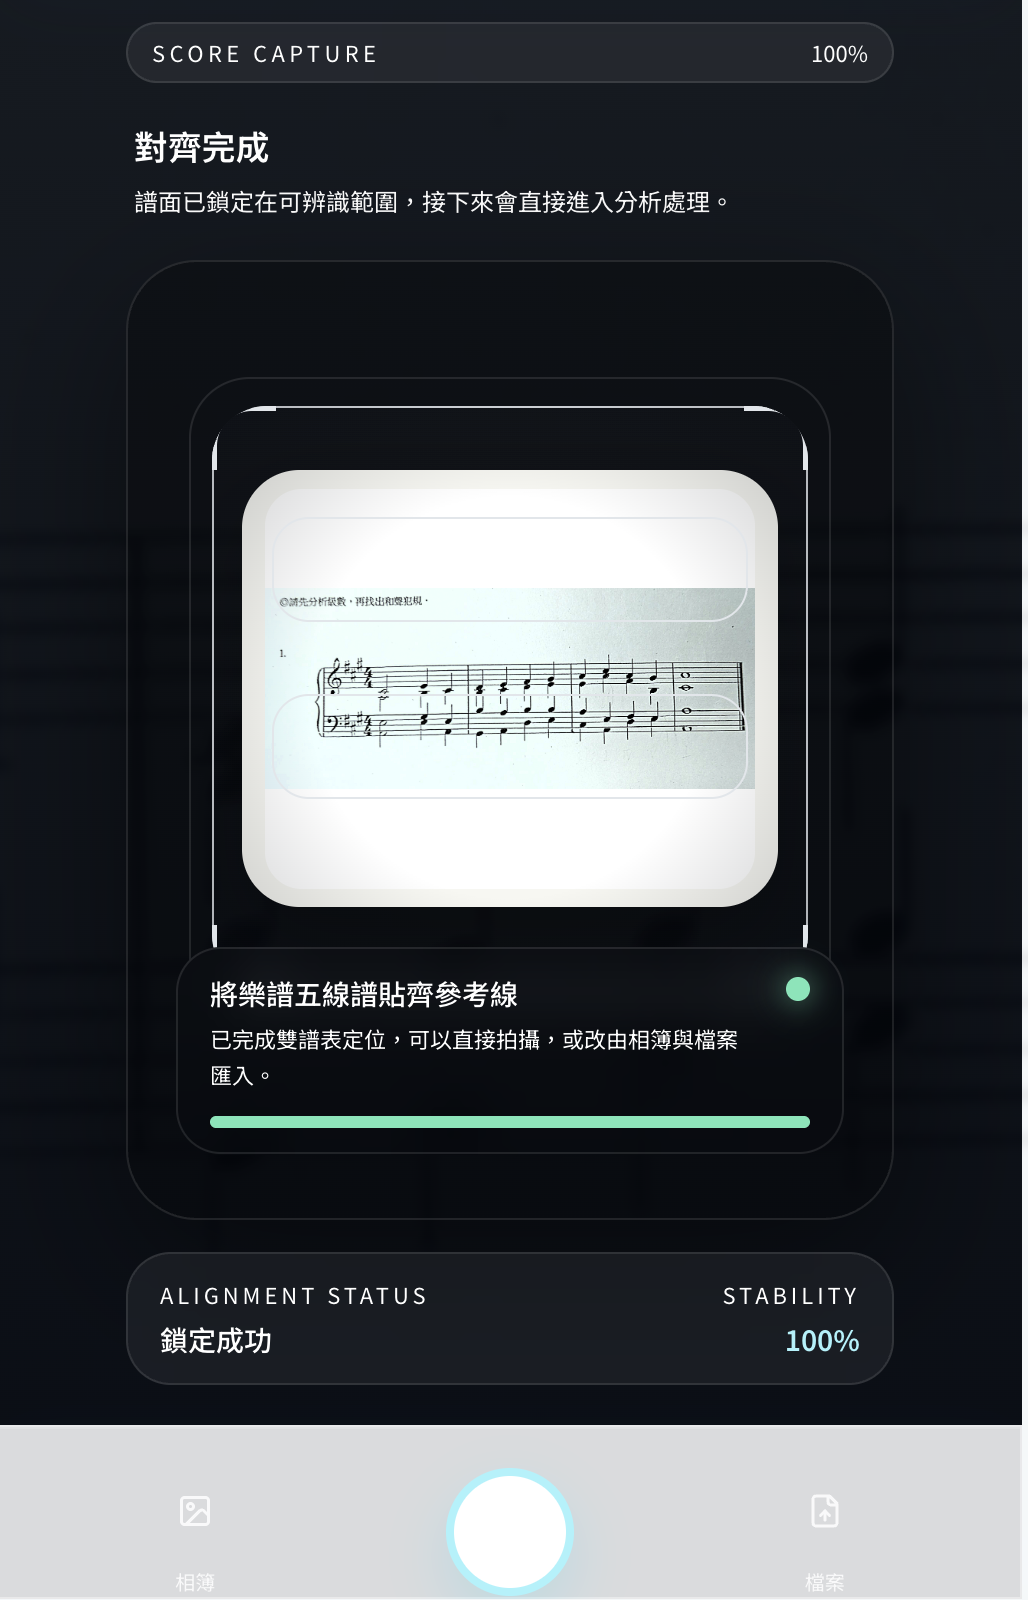
\includegraphics[width=\linewidth,height=6.8cm,keepaspectratio]{figures/prototype_score_capture.png}}
{\fbox{\parbox[c][6.8cm][c]{0.90\linewidth}{\centering Score capture}}}
\scriptsize\textbf{(a) Score capture and alignment}
\end{minipage}
\hfill
\begin{minipage}[t]{0.34\linewidth}
\centering
\IfFileExists{figures/prototype_recognition_review.png}
{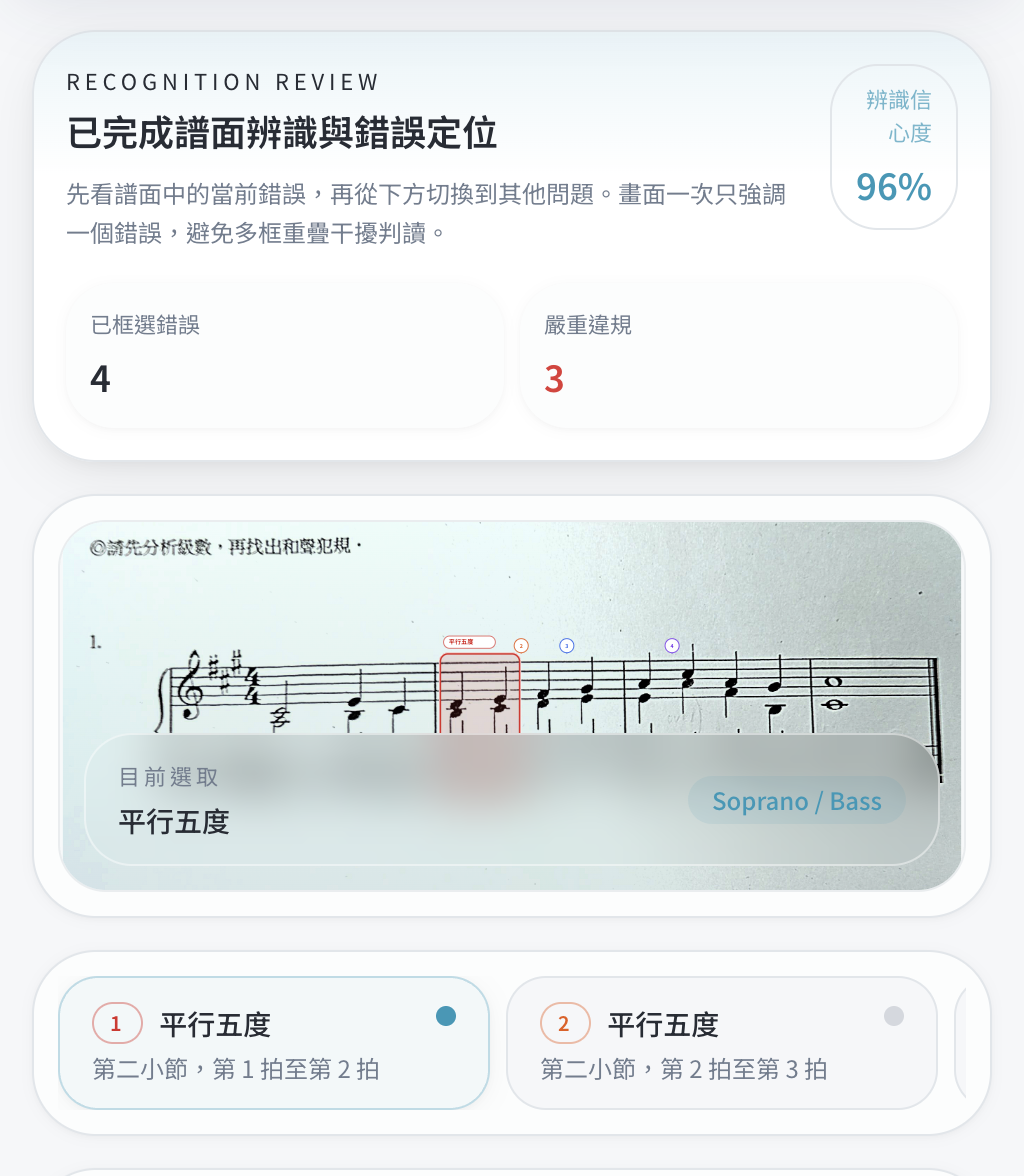
\includegraphics[width=\linewidth,height=6.8cm,keepaspectratio]{figures/prototype_recognition_review.png}}
{\fbox{\parbox[c][6.8cm][c]{0.90\linewidth}{\centering Recognition review}}}
\scriptsize\textbf{(b) Recognition review and error localization}
\end{minipage}
\hfill
\begin{minipage}[t]{0.30\linewidth}
\centering
\IfFileExists{figures/prototype_issue_detail.png}
{
\includegraphics[width=\linewidth,height=6.8cm,keepaspectratio]{figures/prototype_issue_detail.png}}
{\fbox{\parbox[c][6.8cm][c]{0.90\linewidth}{\centering Issue detail}}}
\scriptsize\textbf{(c) Rule explanation and feedback}
\end{minipage}

\vspace{0.08cm}
\scriptsize
\captionof{figure}{Prototype screens showing score capture, recognition review, localized error selection, and rule-based correction feedback.}
\end{center}

\vspace{0.10cm}
The web-based prototype demonstrates the complete user-facing workflow: score
input, recognition progress, error localization, rule explanation, and
correction guidance.
}

\block{{\sectionbar{OMR Model Performance}}}{
\footnotesize
The current best OMR model is based on YOLO12s Ultimate v5 Stable and is
evaluated on a cleaned validation set.

\vspace{0.04cm}
\begin{center}
\scriptsize
\begin{tabular}{lrrrr}
\toprule
\textbf{Metric} & mAP50 & mAP50--95 & Precision & Recall \\
\midrule
\textbf{Result} & 0.7763 & 0.7320 & 0.957 & 0.576 \\
\bottomrule
\end{tabular}
\captionof{table}{OMR detection performance under the deployment protocol.}
\end{center}

\vspace{0.03cm}
\textbf{Observation.}
High precision indicates reliable detections, while recall improvement remains
the main training target, especially for small or rare notation symbols.
}


\block{{\sectionbar{Discussion \& Limitations}}}{
\scriptsize
\begin{tabular}{p{0.48\linewidth}p{0.48\linewidth}}
\textbf{Current strengths} & \textbf{Current limitations} \\
\begin{itemize}
    \item The OMR model achieves promising detection precision for music symbols.
    \item The rule engine provides explainable analysis rather than only binary grading.
    \item The prototype interface makes error locations and rule explanations visible to learners.
    \item The modular design allows the OMR model and rule engine to be improved independently.
\end{itemize}
&
\begin{itemize}
    \item Recall remains the main bottleneck of the OMR model.
    \item Symbol-to-voice assembly requires further improvement for arbitrary handwritten scores.
    \item The current rule set focuses on representative four-part harmony errors.
    \item More advanced harmony phenomena, such as non-chord tones and cadence-specific rules, require future expansion.
\end{itemize}
\end{tabular}
}

\block{{\sectionbar{Conclusion \& Future Work}}}{
\scriptsize
This study presents an automatic four-part harmony grading system that integrates
deep learning-based OMR and rule-based harmony analysis. The system detects
music notation symbols from score images, converts them into structured harmony
representations, and provides localized, explainable feedback for common
four-part harmony errors.

\vspace{0.08cm}
\begin{tabular}{p{0.48\linewidth}p{0.48\linewidth}}
\textbf{Future work} & \textbf{Key takeaway} \\
\begin{itemize}
    \item Improve recall for small and rare notation symbols.
    \item Strengthen the conversion from OMR detections to four-voice structures.
    \item Expand the rule set to include non-chord tones and cadence-specific cases.
    \item Deploy the system to a mobile application for real-time classroom use.
\end{itemize}
&
\setlength{\fboxsep}{4pt}%
\fcolorbox{blue!55!black}{blue!6}{%
    \parbox{0.90\linewidth}{\scriptsize
    The system does not search for a single correct answer; it detects
    violations of harmony rules and provides explainable learning feedback.}%
}
\end{tabular}
}

\block{{\sectionbar{References}}}{
    \scriptsize
    \begin{center}
        \mbox{}\vspace{-1\baselineskip}
        \printbibliography[heading=none]
    \end{center}
}

\end{columns}

\end{document}
